\begin{comment}
\section{Binder}
안드로이드에서 프로세스 간 통신은 Binder IPC를 통한다.\\
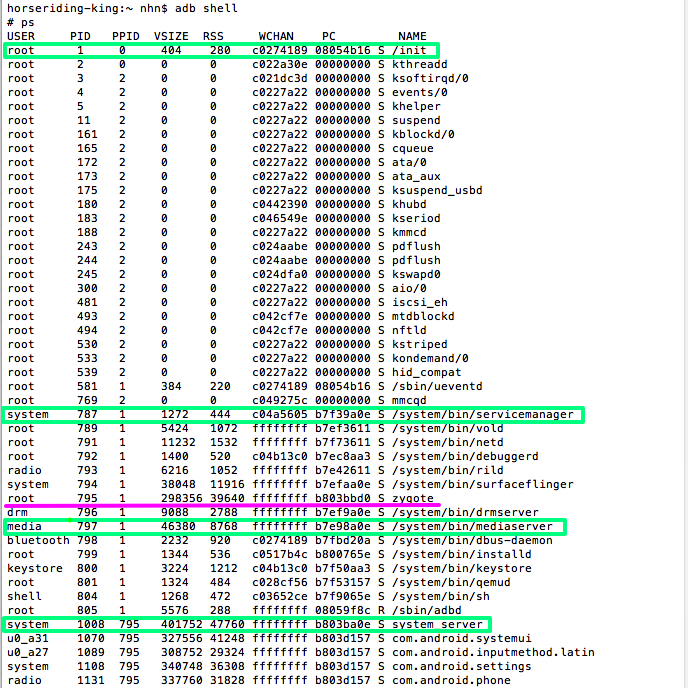
\includegraphics[scale=0.7]{ps}
Binder의 기본 내용은 \url{http://helloworld.naver.com/helloworld/47656}에 간략하게 나와있다.
책으로는 위키북스에서 나온 ``인사이드 안드로이드''나 한빛미디어에서 나온 ``안드로이드의 모든 것 분석과 포팅''을 참고해 보자.\\
Binder IPC, Binder RPC 헷갈린다.

%http://www.angryredplanet.com/~hackbod/openbinder/docs/html/BinderIPCMechanism.html
%http://rts.lab.asu.edu/web_438/project_final/Talk%208%20AndroidArc_Binder.pdf

시스템 서비스는 항상 바인더 통신을 한다.


binder call back 서비스 만들어보자.



% https://thenewcircle.com/s/post/1340/Deep_Dive_Into_Binder_Presentation.htm

binder Thread Pool은 최대 16개. 시작하면서 2개가 생성이 되고(ViewRootImpl, ActivityThread\$ApplicationThread 용도) 필요하면 추가한다. binding이 많다면 timeout 날 수 있다.
/frameworks/native/libs/binder/ProcessState.cpp에서 open\_driver 함수를 보자.
(ZygoteInit.main이 실행되고, RuntimeInit.ZygoteInitNative에서 app\_main.cpp에서 AppRuntiume.onZygoteInit에서 호출한다.)
surfaceflinger는 최대 4개로 세팅하고 있다.(setThreadPollMaxTheadCount 함수 호출)

stub 호출시 handler를 주로 사용한다.(UI 업데이트 필요할 때)
클라이언트는 proxy, 서버는 stub이다.
systemserver: ActivityManagerService, PackageManagerService, LocationManagerService, AlarmManagerService, ConnectivityService, SensorService, WifiService
/system/bin/mediaserver : AudioFlinger, CameraService, MediaPlayerService, AudioPolicyService 네이티브 시스템 서비스로 cpp로 되어 있다.
/system/bin/surfaceflinger: SurfaceFlinger 네이티브 시스템 서비스로 cpp로 되어 있다. 

init.rc에 보면 surfaceflinger가 먼저 실행되고, mediaserver가 실행된다.
systemserver는 zygote에서 실행
servicemanager
\end{comment}
\chapter{시스템 서비스}
% http://www.vogella.com/tutorials/AndroidServices/article.html
%안드로이드에서는 API와 internal에서 시스템 서비스를 구분하는 것이 약간 차이가 있다. 두 가지를 동일한 것으로 이해하고 있다면 혼동이 생기므로, 차이를 정리하고 넘어가도록 하자.
시스템 서비스는 우리가 만드는 Service처럼 따로 실행할 필요가 없고, 시스템에서 이미 존재하고 실행중인 서비스를 앱에서 이용하는 것이다.
일반적으로 시스템 서비스는 자바 시스템 서비스와 네이티브 시스템 서비스 두 그룹으로 분류한다.\\

아래는 adb shell에서 ps 실행 결과이다.\\
\begin{lstlisting}[frame=single] 
shell@EF56S:/ $ ps
USER     PID   PPID  VSIZE  RSS     WCHAN    PC         NAME
root      1     0     788    600   ffffffff 00000000 S /init
root      2     0     0      0     ffffffff 00000000 S kthreadd
root      3     2     0      0     ffffffff 00000000 S ksoftirqd/0
root      6     2     0      0     ffffffff 00000000 D kworker/u:0
root      7     2     0      0     ffffffff 00000000 D kworker/u:0H
root      8     2     0      0     ffffffff 00000000 S migration/0
root      21    2     0      0     ffffffff 00000000 S khelper
root      22    2     0      0     ffffffff 00000000 S netns
root      28    2     0      0     ffffffff 00000000 S modem_notifier
root      29    2     0      0     ffffffff 00000000 S smd_channel_clo
root      30    2     0      0     ffffffff 00000000 S smsm_cb_wq
root      32    2     0      0     ffffffff 00000000 S rpm-smd
root      33    2     0      0     ffffffff 00000000 S kworker/u:1H
root      34    2     0      0     ffffffff 00000000 S mpm
root      49    2     0      0     ffffffff 00000000 S sync_supers
root      50    2     0      0     ffffffff 00000000 S bdi-default
root      51    2     0      0     ffffffff 00000000 S kblockd
root      52    2     0      0     ffffffff 00000000 S system
root      53    2     0      0     ffffffff 00000000 S khubd
...
root      340   1     1484   4     ffffffff 00000000 S /sbin/healthd
system    341   1     1428   588   ffffffff 00000000 S /system/bin/servicemanager
root      342   1     4892   808   ffffffff 00000000 S /system/bin/vold
system    344   1     2568   724   ffffffff 00000000 S /system/bin/rfs_access
system    347   1     3820   1044  ffffffff 00000000 S /system/bin/qseecomd
root      350   1     10648  1488  ffffffff 00000000 S /system/bin/netd
root      351   1     8020   1052  ffffffff 00000000 S /system/bin/debuggerd
root      352   1     1448   580   ffffffff 00000000 S /system/bin/pam_server
radio     353   1     27984  3052  ffffffff 00000000 S /system/bin/rild
system    354   1     121284 5324  ffffffff 00000000 S /system/bin/surfaceflinger
root      355   1     861344 19116 ffffffff 00000000 S zygote
drm       356   1     28192  2748  ffffffff 00000000 S /system/bin/drmserver
media     357   1     69708  7484  ffffffff 00000000 S /system/bin/mediaserver
install   358   1     1412   704   ffffffff 00000000 S /system/bin/installd
keystore  360   1     3736   872   ffffffff 00000000 S /system/bin/keystore
...
shell     477   1     5700   244   ffffffff 00000000 S /sbin/adbd
...
system    1192  355   1014224 74416 ffffffff 00000000 S system_server
u0_a12    1385  355   1082344 150852 ffffffff 00000000 S com.android.systemui
radio     1619  355   913032 24116 ffffffff 00000000 S com.android.phone
u0_a134   1661  355   870396 21168 ffffffff 00000000 S com.skt.tbmon
u0_a50    1675  355   870900 20432 ffffffff 00000000 S com.skt.apra
system    1727  355   872452 18660 ffffffff 00000000 S com.qualcomm.services.location
nfc       1739  355   883544 20352 ffffffff 00000000 S com.android.nfc
system    1753  355   869324 16212 ffffffff 00000000 S com.qualcomm.wfd.service:wfd_service
u0_a110   1780  355   960648 126336 ffffffff 00000000 S com.pantech.launcher2
u0_a197   1881  355   869196 16148 ffffffff 00000000 S com.android.smspush
u0_a9     1976  355   1068200 37924 ffffffff 00000000 S com.google.android.gms
u0_a9     2011  355   939400 32092 ffffffff 00000000 S com.google.process.gapps
u0_a9     2063  355   948572 36028 ffffffff 00000000 S com.google.process.location
u0_a31    2330  355   881220 21224 ffffffff 00000000 S com.skt.skaf.OA00199800
bluetooth 2667  355   915620 21268 ffffffff 00000000 S com.android.bluetooth
system    2688  355   982224 47708 ffffffff 00000000 S com.pantech.powersaver
u0_a57    3025  355   914296 21860 ffffffff 00000000 S com.android.calendar
u0_a63    3304  355   880016 18668 ffffffff 00000000 S com.skt.iwlan:remote
system    3370  355   877760 24112 ffffffff 00000000 S com.skt.tmode
system    3713  355   872376 16280 ffffffff 00000000 S com.qualcomm.atfwd
u0_a65    4640  355   883112 19772 ffffffff 00000000 S com.android.deskclock
u0_a57    4782  355   887760 21420 ffffffff 00000000 S com.android.calendar:remote
u0_a139   7531  355   873552 21924 ffffffff 00000000 S android.process.acore
u0_a15    12207 355   906192 25548 ffffffff 00000000 S com.android.vending
...
\end{lstlisting}

여기서 /system/bin/mediaserver, /system/bin/surfaceflinger 두 가지가 네이티브 시스템 서비스 프로세스이다. 그리고 system\_server가 자바 시스템 서비스 프로세스이다.

\section{네이티브 시스템 서비스}
네이티브 시스템 서비스는 앱에서 일반적으로 직접 접근해서 사용하지 않는다.
%롤리팝에 추가된 CamearManager가 하나의 예외이다.
/system/bin/mediaserver는 MediaPlayer, MediaRecorder, Camera 같은 클래스에서 접근하거나, AudioService 같은 자바 시스템 서비스에서 접근하는 형태\footnote{AudioService에서는 AudioSystem 클래스를 통해 네이티브에 접근한다.}를 띠고 있다.
/system/bin/surfaceflinger는 WindowManagerService에서 접근해서 화면에 반영하고 있다.

\section{자바 시스템 서비스}
API에서 시스템 서비스라고 부르는 것을 보자. 
Context에 getSystemService(String name) 메서드가 있어서, 리턴 결과는 시스템 서비스를 래핑한 것이고 사용 시에 반드시 캐스팅해서 사용한다.
일반적인 패턴은 클라이언트 Binder Proxy를 래핑하고서 -Manager 식의 네이밍을 가진다. 그리고 -Manager에서는 Stub의 모든 public 메서드를 다 사용할 수 있는 것은 아니다. 예를 들어, ActivityManager에서 startActivity() 메서드를 실행할 수는 없다.\\

아래 표를 보도록 하자. 일반적인 네이밍 패턴에 맞는 것도 많지만 아닌 것도 여럿 있다(롤리팝 기준).
% com.android.server.SystemServer 참고
\newgeometry{left=2cm,bottom=2cm}
\scalebox{0.8}{
\begin{tabular}[fontsize=\tiny]{|l|l|l|l|l|} \hline
Context 상수 & getSystemService 결과 & 인터페이스 & Stub 구현 \\ \hline
ACCESSIBILITY\_SERVICE & AccessibilityManager & IAccessibilityManager & AccessibilityManagerService  \\ \hline
ACCOUNT\_SERVICE & AccountManager & IAccountManager & AccountManagerService \\ \hline
ACTIVITY\_SERVICE & ActivityManager & IActivityManager & ActivityManagerService \\ \hline
ALARM\_SERVICE & AlarmManager & IAlarmManager & AlarmManagerService \\ \hline
APPWIDGET\_SERVICE	& AppWidgetManager & IAppWidgetService & AppWidgetService \\ \hline
APP\_OPS\_SERVICE & AppOpsManager & IAppOpsService & AppOpsService \\ \hline
AUDIO\_SERVICE & AudioManager & IAudioService & AudioService \\ \hline
BATTERY\_SERVICE	 & BatteryManager & IBatteryPropertiesRegistrar & IBatteryPropertiesRegistrar.cpp \\ \hline
BLUETOOTH\_SERVICE & BluetoothAdapter & IBluetoothManager & BluetoothManagerService \\ \hline
CAMERA\_SERVICE & CameraManager & ICameraService & CameraService.cpp \\ \hline 
CAPTIONING\_SERVICE & CaptioningManager & 없음 & ContentResolver 사용 \\ \hline
CLIPBOARD\_SERVICE & ClipboardManager & IClipboard & ClipboardService \\ \hline
CONNECTIVITY\_SERVICE & ConnectivityManager & IConnectivityManager & ConnectivityService \\ \hline
CONSUMER\_IR\_SERVICE & ConsumerIrManager & IConsumerIrService & ConsumerIrService \\ \hline
DEVICE\_POLICY\_SERVICE & DevicePolicyManager & IDevicePolicyManager & DevicePolicyManagerService \\ \hline
DISPLAY\_SERVICE	& DisplayManager & IDisplayManager & DisplayManagerService \\ \hline
DOWNLOAD\_SERVICE & DownloadManager & 없음 & ContentResolver 사용 \\ \hline
DROPBOX\_SERVICE	& DropBoxManager & IDropBoxManagerService &  DropBoxManagerService\\ \hline
INPUT\_METHOD\_SERVICE	 & InputMethodManager & IInputMethodManager & InputMethodManagerService \\ \hline
INPUT\_SERVICE & InputManager & IInputManager & InputManagerService \\ \hline
JOB\_SCHEDULER\_SERVICE & JobScheduler & IJobScheduler & JobSchedulerService \\ \hline
KEYGUARD\_SERVICE	 & KeyguardManager & 없음 & 없음 \\ \hline
LAUNCHER\_APPS\_SERVICE & LauncherApps &  ILauncherApps & LauncherAppsService \\ \hline
LAYOUT\_INFLATER\_SERVICE & LayoutInflater & 없음 & 없음 \\ \hline
LOCATION\_SERVICE	 & LocationManager & ILocationManager & LocationManagerService \\ \hline
MEDIA\_PROJECTION\_SERVICE	 & MediaProjectionManager  & IMediaProjectionManager & MediaProjectionManagerService \\ \hline
MEDIA\_ROUTER\_SERVICE	 & MediaRouter & IMediaRouterService & MediaRouterService \\ \hline
MEDIA\_SESSION\_SERVICE & MediaSessionManager & ISessionManager & MediaSessionService\\ \hline
NFC\_SERVICE	& NfcManager & 없음 & 없음 \\ \hline
NOTIFICATION\_SERVICE & NotificationManager & INotificationManager & NotificationManagerService \\ \hline
NSD\_SERVICE	& NsdManager & INsdManager & NsdService \\ \hline
POWER\_SERVICE & PowerManager & IPowerManager & PowerManagerService \\ \hline
PRINT\_SERVICE &	PrintManager & IPrintManager & PrintManagerService\\ \hline
RESTRICTIONS\_SERVICE & RestrictionsManager &  IRestrictionsManager  & RestrictionsManagerService \\ \hline
SEARCH\_SERVICE & SearchManager & ISearchManager & SearchManagerService \\ \hline
SENSOR\_SERVICE & SensorManager & 없음 & 없음 \\ \hline
STORAGE\_SERVICE	& StorageManager & IMountService & MountService\\ \hline
TELECOM\_SERVICE	& TelecomManager &  ITelecomService &  TelecomServiceImpl\\ \hline
TELEPHONY\_SERVICE & TelephonyManager & ITelephonyRegistry & TelephonyRegistry \\ \hline
TEXT\_SERVICES\_MANAGER\_SERVICE & TextServicesManager & ITextServicesManager & TextServicesManagerService \\ \hline
TV\_INPUT\_SERVICE	 & TvInputManager &  ITvInputManager & TvInputManagerService \\ \hline
UI\_MODE\_SERVICE	& UiModeManager & IUiModeManager & UiModeManagerService \\ \hline
USB\_SERVICE	 & UsbManager & IUsbManager & UsbService \\ \hline
USER\_SERVICE	 & UserManager & IUserManager & UserManagerService \\ \hline
VIBRATOR\_SERVICE & Vibrator & IVibratorService & VibratorService \\ \hline
WALLPAPER\_SERVICE & WallpaperManager & IWallpaperManager & WallpaperManagerService \\ \hline
WIFI\_P2P\_SERVICE	 & WifiP2pManager & IWifiP2pManager & WifiP2pService \\ \hline
WIFI\_SERVICE & WifiManager & IWifiManager & WifiService \\ \hline
WINDOW\_SERVICE & WindowManager & IWindowManager & WindowManagerService \\ \hline
\end{tabular}
}
\restoregeometry

4.X 이후에도 여러 서비스가 추가되어서 생소한 것들이 있는데 굳이 살펴보지는 않겠다.
하나하나 보는 것보다는 전체적으로 특기할 만한 내용 위주로 보도록 하자.
\begin{itemize}
\item getSystemService()의 결과로서 -Manager 네이밍을 따르지 않는 것은 JobScheduler, LauncherApps, LayoutInflater, MediaRouter, Vibrator 네 가지이다. 
\item 인터페이스 이름은 getSystemService() 결과 클래스에 일반적으로는 앞에 I를 붙이지만, 예외 케이스가 너무 많다. Manager 자리에 Service가 붙기도 하고, Manager가 빠지기도 하고 ManagerService로 끝나기도 한다. 
\item 시스템 서비스 가운데 가장 많이 참고해야 하는 ActivityManagerService는 추상 클래스인 ActivityActivityManagerNative를 상속한다. ActivityActivityManagerNative는 IActivityManager의 Stub 구현이 아니라, Binder를 상속한 IActivityManager 인터페이스 구현이다. 그래서 asInterface()나 onTransact() 메서드 등이 직접 구현되어 있다.
\item LayoutInflator는 Binder 통신을 하는 것이 아니고, PolicyManager.makeNewLayoutInflater()를 통해  com.android.internal.policy.impl.PhoneLayoutInflator를 가져온다.
LayoutInflator를 가져오는 메서드는 세 가지가 있다.
\begin{itemize}
\item (LayoutInflator) Context.getSystemService(Context.LAYOUT\_INFLATER\_SERVICE)
\item LayoutInflator.from(Context context)
\item Activity의 getLayoutInflator()
\end{itemize}
두 번째와 세 번째가 내부적으로 첫 번째 메서드를 다시 호출하고 있는데, 일반적으로 간편하게 많이 사용하는 것은 두 번째 메서드이다.
\item CameraService는 네이티브로 되어 있다. Binder 통신은 마샬링, 언마샬링만 하면 되기 때문에 네이티브에서 언마샬링해서 요청을 처리하는 식이다.
\item BatteryManager는 기존에는 ACTION\_BATTERY\_CHANGED Intent에서 쓰이는 문자열과 상수만을 정의하고 있었는데, 롤리팝에서 배터리와 충전 속성을 조회하는 메서드가 추가되었다.
\item DownloadService는 별도 프로세스인 android.process.media에서 실행된다. DownloadManager는 ContentResolver를 통해 DB에 쌓는 역할만 한다.
DownloadService 위치는 프레임워크 소스상에서 packages/providers/DownloadProvider 디렉터리에 있고, Service를 상속한 일반 Service이다. 
DownloadReceiver에서 Intent.ACTION\_BOOT\_COMPLETED, Intent.ACTION\_MEDIA\_MOUNTED, ConnectivityManager.CONNECTIVITY\_ACTION(연결될 때)와 내부적으로 쓰는 Action인 ACTION\_RETRY Broadcast 이벤트 발생 시에 DownloadService를 시작한다.
\item SensorManager는 실제 구현은 android.hardware.SystemSensorManager이다. ContextImpl에서 처음 SensorManager를 Service Map에 넣을 때 네이티브에서 Sensor 목록을 로딩해 놓는다.
\item NfcManager는 NfcAdapter를 얻기 위한 용도이다.  getDefaultAdapter() 메서드 하나만 있다. NfcService의 내부클래스인 NfcAdapterService에서 INfcAdapter.Stub을 구현하고, NfcAdapter에서는 여기에 접근한다.
\item 롤리팝에는 com.android.server.SystemService가 추가되어서 Service 클래스는 이를 상속하고 Stub 구현은 내부 클래스에서 하고 있다.\\
\begin{tabular}[fontsize=\tiny]{|l|l|} \hline
Service & Stub 구현 내부 클래스 \\ \hline
JobSchedulerService & JobSchedulerStub \\ \hline
LauncherAppsService & LauncherAppsImpl \\ \hline
MediaSessionService, & SessionManagerImpl \\ \hline
RestrictionsManagerService & RestrictionsManagerImpl \\ \hline
TvInputManagerService & BinderService \\ \hline
\end{tabular}
\end{itemize}

Binder Stub 구현이 없는 것은 실제로는 Binder 통신을 하는 건 아니다.
서비스명이 DOWNLOAD\_SERVICE나 LAYOUT\_INFLATER\_SERVICE 같은 것은 편의상 시스템 서비스일 뿐이다.\\

Binder Stub 구현은 어느 프로세스에서 돌아가고 있을까? Binder Stub이 각각 따로 프로세스로 실행되는 것이 아닐까 생각할 수도 있지만, 앞에서도 여러 차례 얘기한 system\_server 프로세스에서 실행되고 있다.(예외로 CameraService는 /system/bin/mediaserver 프로세스에서 실행된다.)			
system\_server에서 여러 시스템 서비스를 제공하고, 이를 다른 앱에서 호출하는 것으로 이해하면 된다.\\

여기서 하나 질문을 해보자. 일반 리모트 바인딩 서비스와 안드로이드에서 제공하는 시스템 서비스는 어떻게 다를까?
이 내용을 생각해보면 다음과 같이 정리해볼 수 있다.
\begin{itemize}
\item 시스템 서비스는 /system/bin/servicemanager에 Stub을 등록하고 필요할 때 가져와서 사용하고, 일반 서비스는 ActivityManagerService의 내부 목록으로 유지된다.
\item 시스템 서비스는 일반적으로 Stub 자체로 구현하지만, 일반 서비스는 android.os.Service를 상속하고 내부에 Stub을 구현한다.
\end{itemize}

이제 프레임워크 소스를 보도록 하자.
/system/bin/servicemanager 프로세스에 Stub을 등록하는 내용은 /frameworks/base/services/java/com/android/server/SystemServer.java\footnote{system\_server 프로세스의 메인 클래스이다.}에서 내부 클래스인 ServerThread의 initAndLoop() 메서드에서 볼 수 있다.

\begin{lstlisting}[frame=single, caption=SystemServer.java] 
	    display = new DisplayManagerService(context, wmHandler);
	    ServiceManager.addService(Context.DISPLAY_SERVICE, display, true);
	
	    telephonyRegistry = new TelephonyRegistry(context);
	    ServiceManager.addService("telephony.registry", telephonyRegistry);
	
	    ServiceManager.addService("scheduling_policy", new SchedulingPolicyService());
		
		...
		ActivityManagerService.setSystemProcess(); // (1)
		
		...
	    ServiceManager.addService("battery", battery);
	
	    vibrator = new VibratorService(context);
	    ServiceManager.addService("vibrator", vibrator);
	
		...
	    inputManager = new InputManagerService(context, wmHandler);
	    wm = WindowManagerService.main(context, power, display, inputManager,
	            wmHandler, factoryTest != SystemServer.FACTORY_TEST_LOW_LEVEL,
	            !firstBoot, onlyCore);
	    ServiceManager.addService(Context.WINDOW_SERVICE, wm);
	    ServiceManager.addService(Context.INPUT_SERVICE, inputManager);
\end{lstlisting}	    
ServiceManager.addService() 메서드를 통해서 여러 Stub을 등록하는 것을 볼 수 있다.
% /frameworks/base/core/java/android/os/ServiceManager.java
여기서 보면 ActivityManagerService 등록이 눈에 띄지 않는데, 관련 코드는 ActivityManagerService 안에 있다. 10라인(1)에서 ActivityManagerService.setSystemProcess() 호출이 있는데, 여기서 자기 자신을 등록하고 있다.\\
\begin{lstlisting}[frame=single, caption=ActivityManagerService.java] 
   public static void setSystemProcess() {
        try {
            ActivityManagerService m = mSelf;

            ServiceManager.addService(Context.ACTIVITY_SERVICE, m, true);
            ServiceManager.addService(ProcessStats.SERVICE_NAME, m.mProcessStats);
            ServiceManager.addService("meminfo", new MemBinder(m));
            ServiceManager.addService("gfxinfo", new GraphicsBinder(m));
            ServiceManager.addService("dbinfo", new DbBinder(m));
            if (MONITOR_CPU_USAGE) {
                ServiceManager.addService("cpuinfo", new CpuBinder(m));
            }
            ServiceManager.addService("permission", new PermissionController(m));
 			...
        } catch (PackageManager.NameNotFoundException e) {
            throw new RuntimeException(
                    "Unable to find android system package", e);
        }
    }
\end{lstlisting}	    


\begin{comment}
ViewRootImpl에서 onConfigurationChanged 이후에 measure 호출하고 있다. 사이즈 조정하기 좋은 곳이 onConfigurationChanged 메서드이다.

ActivityManagerService, WindowManagerService, PackageManagerService, LocationManagerService, AlarmManagerService, PowerManagerService, BackupManagerService, InputManagerService, AppWidgetService, AudioService, ConnectivityService, VibratorService 등 자바 시스템 서비스로 Binder Stub을 구현하고 있고, system\_server 프로세스에서 실행된다.\\
\end{comment}

시스템 서비스를 사용하는 쪽에서는 어떨까. 매번 /system/bin/servicemanager에서 조회해서 호출하는가 하면 그렇지 않다.
바로 ContextImpl의 정적 초기화 블록(static initializer block) 안에서 처음 생성될 때 단 한번만 매핑하고 사용한다.
\begin{lstlisting}[frame=single, caption=ContextImpl.java] 
  private static final HashMap<String, ServiceFetcher> SYSTEM_SERVICE_MAP =
            new HashMap<String, ServiceFetcher>();

  private static int sNextPerContextServiceCacheIndex = 0;
  private static void registerService(String serviceName, ServiceFetcher fetcher) {
      if (!(fetcher instanceof StaticServiceFetcher)) {
          fetcher.mContextCacheIndex = sNextPerContextServiceCacheIndex++;
      }
      SYSTEM_SERVICE_MAP.put(serviceName, fetcher);
  }
    
  static {
        registerService(ACCESSIBILITY_SERVICE, new ServiceFetcher() {
                public Object getService(ContextImpl ctx) {
                    return AccessibilityManager.getInstance(ctx);
                }});

        registerService(ACCOUNT_SERVICE, new ServiceFetcher() {
                public Object createService(ContextImpl ctx) {
                    IBinder b = ServiceManager.getService(ACCOUNT_SERVICE);
                    IAccountManager service = IAccountManager.Stub.asInterface(b);
                    return new AccountManager(ctx, service);
                }});

        registerService(ACTIVITY_SERVICE, new ServiceFetcher() {
                public Object createService(ContextImpl ctx) {
                    return new ActivityManager(ctx.getOuterContext(), ctx.mMainThread.getHandler());
                }});

        registerService(ALARM_SERVICE, new ServiceFetcher() {
                public Object createService(ContextImpl ctx) {
                    IBinder b = ServiceManager.getService(ALARM_SERVICE);
                    IAlarmManager service = IAlarmManager.Stub.asInterface(b);
                    return new AlarmManager(service, ctx);
                }});
		....
        registerService(LAYOUT_INFLATER_SERVICE, new ServiceFetcher() {
                public Object createService(ContextImpl ctx) {
                    return PolicyManager.makeNewLayoutInflater(ctx.getOuterContext());
                }});

        registerService(LOCATION_SERVICE, new ServiceFetcher() {
                public Object createService(ContextImpl ctx) {
                    IBinder b = ServiceManager.getService(LOCATION_SERVICE);
                    return new LocationManager(ctx, ILocationManager.Stub.asInterface(b));
                }});

        registerService(NETWORK_POLICY_SERVICE, new ServiceFetcher() {
            @Override
            public Object createService(ContextImpl ctx) {
                return new NetworkPolicyManager(INetworkPolicyManager.Stub.asInterface(
                        ServiceManager.getService(NETWORK_POLICY_SERVICE)));
            }
        });

        registerService(NOTIFICATION_SERVICE, new ServiceFetcher() {
                public Object createService(ContextImpl ctx) {
                    final Context outerContext = ctx.getOuterContext();
                    return new NotificationManager(
                        new ContextThemeWrapper(outerContext,
                                Resources.selectSystemTheme(0,
                                        outerContext.getApplicationInfo().targetSdkVersion,
                                        com.android.internal.R.style.Theme_Dialog,
                                        com.android.internal.R.style.Theme_Holo_Dialog,
                                        com.android.internal.R.style.Theme_DeviceDefault_Dialog)),
                        ctx.mMainThread.getHandler());
                }});

        registerService(POWER_SERVICE, new ServiceFetcher() {
                public Object createService(ContextImpl ctx) {
                    IBinder b = ServiceManager.getService(POWER_SERVICE);
                    IPowerManager service = IPowerManager.Stub.asInterface(b);
                    return new PowerManager(ctx.getOuterContext(),
                            service, ctx.mMainThread.getHandler());
                }});
		....
        registerService(TELEPHONY_SERVICE, new ServiceFetcher() {
                public Object createService(ContextImpl ctx) {
                    return new TelephonyManager(ctx.getOuterContext());
                }});

        registerService(VIBRATOR_SERVICE, new ServiceFetcher() {
                public Object createService(ContextImpl ctx) {
                    return new SystemVibrator(ctx);
                }});
		....
    }
\end{lstlisting}
AccountManager나 AlarmManager를 보면 Binder Proxy를 감싼 객체임을 바로 알수 있는데, 대부분 이와 유사하게 되어 있다.\\

% http://developer.android.com/reference/android/content/Context.html

\section{dumpsys 명령어}\label{sec:dumpsys}
adb shell에서 가장 많이 실행하는 명령어 가운데 하나가 앞에서도 여러 차례 언급한 dumpsys이다. 
dumpsys만을 쓰면 너무 많은 정보가 나오고, dumpsys activity나 dumpsys package 처럼 원하는 정보에 한정해서 보는 것이 좋다.
그런데 dumpsys 다음에 들어가는 옵션 항목은 어떤 것이 있을까? 이를 아는 방법은 바로 shell에서 service list\footnote{/frameworks/native/cmds/service/service.cpp에 있다.}를 실행하는 것이다.
% Android Graphics Architecture.pdf 참고할 것
\begin{lstlisting}[frame=single] 
# service list
Found 65 services:
0	phone: [com.android.internal.telephony.ITelephony]
1	iphonesubinfo: [com.android.internal.telephony.IPhoneSubInfo]
2	simphonebook: [com.android.internal.telephony.IIccPhoneBook]
3	isms: [com.android.internal.telephony.ISms]
4	commontime_management: []
5	samplingprofiler: []
6	diskstats: []
7	appwidget: [com.android.internal.appwidget.IAppWidgetService]
8	backup: [android.app.backup.IBackupManager]
9	uimode: [android.app.IUiModeManager]
10	serial: [android.hardware.ISerialManager]
11	usb: [android.hardware.usb.IUsbManager]
12	audio: [android.media.IAudioService]
13	wallpaper: [android.app.IWallpaperManager]
14	dropbox: [com.android.internal.os.IDropBoxManagerService]
15	search: [android.app.ISearchManager]
16	country_detector: [android.location.ICountryDetector]
17	location: [android.location.ILocationManager]
18	devicestoragemonitor: []
19	notification: [android.app.INotificationManager]
20	updatelock: [android.os.IUpdateLock]
21	throttle: [android.net.IThrottleManager]
22	servicediscovery: [android.net.nsd.INsdManager]
23	connectivity: [android.net.IConnectivityManager]
24	wifi: [android.net.wifi.IWifiManager]
25	wifip2p: [android.net.wifi.p2p.IWifiP2pManager]
26	netpolicy: [android.net.INetworkPolicyManager]
27	netstats: [android.net.INetworkStatsService]
28	textservices: [com.android.internal.textservice.ITextServicesManager]
29	network_management: [android.os.INetworkManagementService]
30	clipboard: [android.content.IClipboard]
31	statusbar: [com.android.internal.statusbar.IStatusBarService]
32	device_policy: [android.app.admin.IDevicePolicyManager]
33	lock_settings: [com.android.internal.widget.ILockSettings]
34	mount: [IMountService]
35	accessibility: [android.view.accessibility.IAccessibilityManager]
36	input_method: [com.android.internal.view.IInputMethodManager]
37	input: [android.hardware.input.IInputManager]
38	window: [android.view.IWindowManager]
39	alarm: [android.app.IAlarmManager]
40	vibrator: [android.os.IVibratorService]
41	battery: []
42	hardware: [android.os.IHardwareService]
43	content: [android.content.IContentService]
44	account: [android.accounts.IAccountManager]
45	permission: [android.os.IPermissionController]
46	cpuinfo: []
47	dbinfo: []
48	gfxinfo: []
49	meminfo: []
50	activity: [android.app.IActivityManager]
51	package: [android.content.pm.IPackageManager]
52	scheduling_policy: [android.os.ISchedulingPolicyService]
53	telephony.registry: [com.android.internal.telephony.ITelephonyRegistry]
54	usagestats: [com.android.internal.app.IUsageStats]
55	batteryinfo: [com.android.internal.app.IBatteryStats]
56	power: [android.os.IPowerManager]
57	entropy: []
58	sensorservice: [android.gui.SensorServer]
59	media.audio_policy: [android.media.IAudioPolicyService]
60	media.camera: [android.hardware.ICameraService]
61	media.player: [android.media.IMediaPlayerService]
62	media.audio_flinger: [android.media.IAudioFlinger]
63	SurfaceFlinger: [android.ui.ISurfaceComposer]
64	drm.drmManager: [drm.IDrmManagerService]
\end{lstlisting}

clone(:) 앞에 있는 문자열이 바로 dumpsys 다음에 올 수 있는 값들이다.
이 항목들이 dump할 수 있다는 것인데, 이 항목들은 무엇인가 하면 /system/bin/servicemanager에 등록된 시스템 서비스 목록이다.
항목의 어떤 내용을 출력하는지는 ActivityManagerService, AlarmManagerService 등 시스템 서비스 클래스의 dump() 메서드를 보면 된다. 앞에서 안드로이드 버전마다 dumpsys 결과가 차이가 있다고 언급하였는데, 버전이 올라가면서 dump() 메서드는 클래스에 새로 추가된 여러 멤버 변수값과 함께 더 상세한 내용을 출력하고 있다.\\

service list 결과에서 clone(:) 뒤에 [] 공백으로 나오는 것은 Binder Stub을 등록한 것이 아닌 Binder를 만들어서 일부러 등록한 것이다. dump 용도의 서비스가 등록된 것이다.
dumpsys meminfo 같은 명령을 쓰는 경우가 있는데, meminfo 관련 시스템 서비스는 없다. 위에서 ActivityManagerService.setSystemProcess() 메서드 7라인을 보면 ServiceManager.addService(``meminfo'', new MemBinder(m))가 있다.
이제 ActivityManagerService의 정적 내부 클래스인 MemBinder를 찾아보면 별 게 없고, Binder를 상속하고 dump() 메서드가 유일한 메서드일 뿐이다.
\begin{lstlisting}[frame=single]
    static class MemBinder extends Binder {
        ActivityManagerService mActivityManagerService;
        MemBinder(ActivityManagerService activityManagerService) {
            mActivityManagerService = activityManagerService;
        }

        @Override
        protected void dump(FileDescriptor fd, PrintWriter pw, String[] args) {
            if (mActivityManagerService.checkCallingPermission(android.Manifest.permission.DUMP)
                    != PackageManager.PERMISSION_GRANTED) {
                pw.println("Permission Denial: can't dump meminfo from from pid="
                        + Binder.getCallingPid() + ", uid=" + Binder.getCallingUid()
                        + " without permission " + android.Manifest.permission.DUMP);
                return;
            }

            mActivityManagerService.dumpApplicationMemoryUsage(fd, pw, "  ", args, false, null);
        }
    }
\end{lstlisting}
이것이 동작하는 이유는 Binder에도 기본적으로 onTransact() 메서드가 정의되어 있고,
여기서 DUMP\_TRANSAC\-TION code에 대해 처리하기 때문이다.
그리고 시스템 서비스 Stub에서는 onTransact() 메서드 맨 아래에 super.onTransact(code, data, reply, flags)를 호출하고 있다.

\begin{lstlisting}[frame=single]
   protected boolean onTransact(int code, Parcel data, Parcel reply,
            int flags) throws RemoteException {
        if (code == INTERFACE_TRANSACTION) {
            reply.writeString(getInterfaceDescriptor());
            return true;
        } else if (code == DUMP_TRANSACTION) {
            ParcelFileDescriptor fd = data.readFileDescriptor();
            String[] args = data.readStringArray();
            if (fd != null) {
                try {
                    dump(fd.getFileDescriptor(), args);
                } finally {
                    try {
                        fd.close();
                    } catch (IOException e) {
                    }
                }
            }
            if (reply != null) {
                reply.writeNoException();
            } else {
                StrictMode.clearGatheredViolations();
            }
            return true;
        }
        return false;
    }
\end{lstlisting}

dumpsys activity를 하면 ActivityManagerService가 워낙 많은 정보를 가지고 있기 때문에 보여주는 것이 적지 않다.
정작 필요한 정보를 찾기 위해서 추가로 명령을 덧붙이는 게 좋다. -h 옵션을 사용해서 추가로 덧붙여 쓸 수 있는 것을 알아보자.(모든 서비스가 -h 옵션을 쓸 수 있는 것은 아니다.)
아래는 activity와 package, meminfo에 쓸 수 있는 것을 조회한 것이다.
\begin{lstlisting}[frame=single]
shell@EF56S:/ $ dumpsys activity -h 
Activity manager dump options:
  [-a] [-c] [-h] [cmd] ...
  cmd may be one of:
    a[ctivities]: activity stack state
    b[roadcasts] [PACKAGE_NAME] [history [-s]]: broadcast state
    i[ntents] [PACKAGE_NAME]: pending intent state
    p[rocesses] [PACKAGE_NAME]: process state
    o[om]: out of memory management
    prov[iders] [COMP_SPEC ...]: content provider state
    provider [COMP_SPEC]: provider client-side state
    s[ervices] [COMP_SPEC ...]: service state
    service [COMP_SPEC]: service client-side state
    package [PACKAGE_NAME]: all state related to given package
    all: dump all activities
    top: dump the top activity
  cmd may also be a COMP_SPEC to dump activities.
  COMP_SPEC may be a component name (com.foo/.myApp),
    a partial substring in a component name, a
    hex object identifier.
  -a: include all available server state.
  -c: include client state.
  
shell@EF56S:/ $ dumpsys package -h                                             
Package manager dump options:
  [-h] [-f] [cmd] ...
    -f: print details of intent filters
    -h: print this help
  cmd may be one of:
    l[ibraries]: list known shared libraries
    f[ibraries]: list device features
    r[esolvers]: dump intent resolvers
    perm[issions]: dump permissions
    pref[erred]: print preferred package settings
    preferred-xml [--full]: print preferred package settings as xml
    prov[iders]: dump content providers
    p[ackages]: dump installed packages
    s[hared-users]: dump shared user IDs
    m[essages]: print collected runtime messages
    v[erifiers]: print package verifier info
    <package.name>: info about given package
    k[eysets]: print known keysets
    
shell@EF56S:/ $ dumpsys meminfo -h
meminfo dump options: [-a] [-d] [-c] [--oom] [process]
  -a: include all available information for each process.
  -d: include dalvik details when dumping process details.
  -c: dump in a compact machine-parseable representation.
  --oom: only show processes organized by oom adj.
  --local: only collect details locally, don't call process.
If [process] is specified it can be the name or 
pid of a specific process to dump.
\end{lstlisting}

Debug 클래스에 dumpService() 메서드도 있다. 이 메서드로 파일에 dumpsys 결과를 출력할 수 있는데, 메서드를 사용하기 위해서는 android.permission.DUMP 퍼미션이 필요하고 이 퍼미션은 시스템 레벨 앱에서만 사용할 수 있다. 따라서 일반 앱에서는 Debug.dumpService()는 사용할 수 없는 메서드이다.

\begin{comment}
코드 상에서도 dump를 생성하고 싶은 경우가 있다.
아래는 안드로이드 소스에서 /packages/apps/Settings 앱에서 Debug.dumpService(String name, FileDescriptor fd, String[] args) 메서드를 사용한 예이다. (android.permission.DUMP 퍼미션은 필요하다.)
\begin{lstlisting}[frame=single]
    ComponentName comp = new ComponentName(mServiceItem.mServiceInfo.packageName,
            mServiceItem.mServiceInfo.name);
    File filename = getActivity().getFileStreamPath("service_dump.txt");
    FileOutputStream output = null;
    try {
        output = new FileOutputStream(filename);
        Debug.dumpService("activity", output.getFD(),
                new String[] { "-a", "service", comp.flattenToString() });
    } catch (IOException e) {
        Log.w(TAG, "Can't dump service: " + comp, e);
    } finally {
        if (output != null) try { output.close(); } catch (IOException e) {}
    }
\end{lstlisting}   
코드 내용은 dumpsys activity -a service 명령 실행 결과를 service\_dump.txt 파일에 출력하는 것이다.
dumpsys activity -a service com.nhn 하면 이렇게 시작하는 서비스 목록이 나온다.

예를 들어 samplingprofiler, battery, commontime\_management, diskstats, entropy 같은 경우는 SystemServer에서 등록하고,
/frameworks/base/services/java/com/android/server/SystemServer.java
meminfo, gfxinfo, dbinfo, cpuinfo 같은 것은 /frameworks/base/services/java/com/android/server/am/ActivityManagerService에서 등록하고, SystemServer에서 ActivitiyManagerService.setSystemProcess를 호출해서 등록한다.

ISurfaceComposer는 자바 소스가 아닌 native cpp 소스이다.
/frameworks/native/libs/gui/아래에 있다.
SurfaceFlinger는 /frameworks/native/services/surfaceflinger/SurfaceFlinger.cpp 이다. 
dumpsys를 해봐도 결과가 없는 것들도 있긴 하다..

등록된 역순으로 나온다. 

앱에서 만드는 Service는 ActivityManager에 등록된다.(/frameworks/base/services/java/com/android/server/am/ActiveServices.java

dumpsys activity services
\end{comment}

\section{시스템 서비스 이슈}
\subsection{빈번한 리모트 호출}
시스템 서비스의 메소드를 호출하는 것은 system\_server 프로세스에 Binder RPC 호출을 하므로, 아무래도 로컬 호출보다는 시스템에 부담을 주게 된다.
그런데 그런 메소드 가운데서 앱에서 빈번하게 호출하는 케이스가 있다.
예를 들어보자. 서버 API를 호출할 때마다 앱의 versionCode를 request parameter나 Header에 전달해야 하는 경우가 있다.(클라이언트 버전의 사용률을 체크하기 위한 용도도 있고, 어느 버전에서 문제가 발생했는지 트래킹하는 데도 쓰인다.)
현재 앱의 버전 정보를 알기 위해서 PackageManager를 통해서 RPC 호출을 해야만 하는데 뭔가 비효율적이긴 하다. 
마치 내 나이를 알기 위해서 꼭 주민센터에 물어봐야 하는 것처럼 말이다. 
Context에는 getPackageName() 메소드는 있지만, getPackageVersionCode() 같은 메소드는 없다.\\

PackageManager를 이용해서 versionCode를 구하는 코드는 아래와 같다.
\begin{lstlisting}[frame=single]
	public static int getAppVersionCode() {
		try {
			return mContext.getPackageManager().getPackageInfo(mContext.getPackageName(), Context.MODE_PRIVATE).versionCode;
		} catch (PackageManager.NameNotFoundException ex) {
			return -1;
		}
	}
\end{lstlisting}

이제 매 호출시마다 getAppVersionCode() 메서드를 호출하는 건 어떨까?
2가지 정도 문제점을 생각할 수 있다.
\begin{itemize}
\item 당연한 얘기지만 빈번한 호출로 부하를 발생시킨다.
\item system\_server도  가끔은 죽을 수 있다. 발생빈도가 낮지만, 시스템 상태가 좋지 않거나 메모리가 부족하다면 가능한 얘기이다. 이때 스택 트레이스에는 ``Caused by: java.lang.RuntimeException: system server dead?'' 메시지를 보여준다. system\_server는 물론 죽자마자 다시 살아나긴 한다.
\end{itemize}

매 호출마다 동일한 값을 리턴하므로, 이 경우에는 불필요한 호출을 줄이기 위해서 메모리(Application 인스턴스의 변수나, 싱글톤 인스턴스에 저장된 값)나 SharedPreferences 사용을 고려할 수 있다(앱 버전을 사용하는 이 경우에 한해서는 최신 IDE에서는 BuildConfig에 생성해주는 VERSION\_CODE, VERSION\_NAME 상수를 사용하는 것도 가능하다).

동일한 결과를 리턴하는 이런 특수한 케이스가 아니더라도 가능하면 리모트 호출을 줄이는 방안을 생각하자. 
시스템 Broadcast를 LocalBroadcastManager로 변경하는 것도 리모트 호출을 줄이는 하나의 예이다. 

\subsection{전원 관리와 Deep Sleep}
이 절에서는 안드로이드의 전원 관리의 기본 내용과 Deep Sleep 이슈에 대해 살펴보자. 마시멜로에서 도입된 Doze Mode에 대해서는 여기서는 다루지 않겠다.\\

모바일 단말은 상시 전원이 차단된 상태로 오랜 시간 사용해야 하므로, 전원 관리는 안드로이드 플랫폼에서 주요 이슈이면서 우리가 만드는 앱에서도 간과해서는 안 되는 문제이다.
안드로이드 Power Management 관련해서 자세한 내용은 `안드로이드 하드웨어 서비스'(개발자가 행복한 세상)을 참고하자.\\

안드로이드 전원 관리 메커니즘은 젤리빈 API 레벨 17 까지는 Wakelock, Early Suspsend, Late Resume 방식을 사용했는데, 리눅스 메인 커널과 통합되는 과정에서(3.4) Autosleep, Wakeup sources로 변경되었다. 내부적으로 방식이 바뀌었지만 앱 개발에서는 동일하게 WakeLock을 잡고 해제하는 코드를 그대로 사용하면 된다.\\

\begin{comment}
먼저 안드로이드 플랫폼의 전원 관리 방법에 대해서 알아보고, 앱에서는 어떤 원칙을 가지고 해야 하는지 살펴보도록 하자.\\

안드로이드 Power Management는 Linux Power Management를 기반으로 한다.
먼저 Linux Kernel의 Power Management를 간단히 얘기해보자.
\begin{itemize}
\item APM(Advanced Power Management)은 BIOS에 기반을 둔 전원 관리 규격이다. APM BIOS에서 APM Driver에 이벤트를 전달하면, APM Driver에서 이벤트에 맞는 전원관리 함수를 한다.
\end{itemize}

Android의 Power Management는 이렇다.
\begin{itemize}
\item BIOS가 없다.
\item 상시 전원이 들어있는 데스크탑과는 달리, 모바일 기기에서는 꺼져있는 상태를 기본으로 하고(Sleep), WakeLock을 통해 필요할 때만 on 시켜서 사용하는 것이 특징이다.
\item  Suspend/Resume 동작을 통해서 Sleep 상태로 이동하고 빠져나오는데, early_suspend, late_resume이 들어간다.
\end{itemize}
\end{comment}

상시 전원이 들어있는 데스크탑과는 달리 모바일 기기에서는 꺼져있는 상태를 기본으로 하고(Sleep), WakeLock을 통해 필요할 때만 ON시켜서 사용하는 것이 특징이다.
Sleep 상태에 들어가면, LCD, Backlight, 카메라, 각종 센서 등의 전원이 차단되고 CPU도 최소 전력 상태로 들어간다.\footnote{최소한의 에너지만 사용하는 겨울잠에 비유되기도 한다.}\\ 

그런데 Sleep은 뭐고 Deep Sleep은 무엇일까? 아무리 찾아봐도 차이에 대한 언급이 별로 없다. 결론적으로 동일한 것으로 보면 된다. 
Sleep에서 깨우는데 소요되는 시간에 따라 Deep Sleep, Deeper Sleep으로 상세하게 구분되는 경우는 있다.\footnote{\url{http://www.intel.com/support/processors/sb/CS-028739.htm}를 참고하자}
Sleep보다 Deep Sleep이라고 언급하는 것이 개념 이해에 도움이 되어서 자주 쓰이는 것 뿐이다. 
깊이(Deep) 잠들어서 아무것도 안 한다는 의미로 이해하자.
필자의 경우에는 Deep Sleep은 특별한 경우에만 발생하는 케이스로 오해했다. 
즉 Sleep과 Deep Sleep을 다른 것으로 생각하고, Deep Sleep은 일반적으로 고려하지 않아도 되는 특수한 상황이 아닐까 했는데, 모바일 단말에서 Deep Sleep은 우리 아주 가까이에 있는 흔한 경우다.\\

앱을 개발하면서 Deep Sleep 상태에서 무엇보다 신경써야 하는 것이 CPU Sleep이다.
Deep Sleep 상태에서는 당연하게도 코드 실행이 중지된다. 메서드 안에 for 문이 실행 중이라면, 끝까지 다 실행하고 Sleep할 것 같은데 잠들 때는 사정없이 잠들어서 코드 실행이 도중에 멈추기도 한다.\\

Deep Sleep 관련해서 안드로이드 개발자 사이트에서 검색하면 나오는 내용이 쓸모 있는 게 거의 없다. 그나마 나오는 결과 가운데서 안드로이드 클래스에서 Deep Sleep 관련해서 살펴볼 게 있다.

\begin{itemize}
\item SystemClock.uptimeMillis() 메소드는 부팅 이후에 Deep Sleep을 제외한 시간을 보여준다. 반면에 SystemClock.elapsedRealtime()은 부팅 이후 (Deep Sleep을 포함한) 시간을 보여준다. 
따라서 elapsedRealtime()에서 uptimeMillis()를 뺀 시간이 바로 Deep Sleep 상태에 있던 시간이다. 처음 부팅을 하고서 화면이 켜진 상태에서는 두 시간이 동일하다. 그 상태에서 화면을 OFF 시키고 몇 분 후에 다시 이 시간 차이를 비교해보자. 그 차이를 따져보면 화면을 OFF 시켰을 때 몇 십초 내에 Deep Sleep 상태로 가는 것을 알 수 있다.
\item Thread.sleep(long time)이나 SystemClock.sleep(long ms) 메소드의 파라미터 값은 Deep Sleep 상태에 있는 시간이 제외된 시간이다. SystemClock.sleep(long ms) 메소드는 InterruptedException을 무시하는 것이 Thread.sleep(long time)과 다르다. 예를 들어, 1분 간 sleep()을 실행하고 다른 작업을 하려고 했는데 sleep() 도중에 Deep Sleep에 빠지면 결과적으로 현상으로 보여지는 sleep 시간은 `1분 + Deep Sleep 상태에 빠진 시간'이다. 
\item Handler에서 postAtTime() 메소드나 postDelayed() 메소드(계산을 통해 내부적으로 postAtTime()을 호출한다.)는 uptimeMillis를 기준으로 한다. 따라서 도중에 Deep Sleep 상태에 들어가면 1분의 Delay를 주었을 뿐이지만, Deep Sleep에서 깨어나고 한참 후에(다른 Message 처리할 것이 앞에 가로막지 않는다면, 최대 1분) 실행될 수도 있다.
% http://stackoverflow.com/questions/17561380/android-thread-sleep-sometimes-waits-far-too-long
\item PowerManager에는 isSleep()이나 isDeepSleep() 같은 메서드는 없다. 이런 메서드는 의미가 없는 게 Deep Sleep 상태에서는 메서드가 실행되지 않을 것이고, 깨어나 있는 상태에서는 이미 Deep Sleep 상태가 아니기 때문이다.
\end{itemize}

이 가운데서 앱을 개발하면서 가장 이슈가 많은 것이 세 번째이다. 
MessageQueue에 Message가 들어갔는데, 실행이 안 되는 것처럼 보이는 케이스가 바로 그것이다.\\

앞에서 반복적으로 UI를 갱신하는 패턴에 대해서 얘기했는데, 이 패턴을 다시 한번 보자.
\begin{lstlisting}[frame=single, caption=Deep Sleep 대응 필요, label=src:DefaultUpdateTime] 
  	private Handler handler = new Handler();

	private static final int DELAY_TIME = 1000;
	private Runnable updateTimeTask = new Runnable() {

		@Override
		public void run() {
			title.setText(new Date().toString());
			handler.postDelayed(this, DELAY_TIME);
		}

	};

	public void onClickButton(View view) {
		handler.post(updateTimeTask);
	}
\end{lstlisting}
1초마다 TextView에 현재 날짜와 시간을 갱신하고 있다.
이런 패턴은 DigitalClock이나 TextClock에서도 쓰이는데 내부적으로 DELAY\_TIME을 1초 이내로 줘서 매 간격마다 시간을 갱신한다. 
우리가 사용하는 단말에서 화면에 나타나는 시계도 이런 형태로 구현되어 있다.
단말을 옆에 한참 방치해놓다가, 화면을 ON하면 순식간에 시간이 한참 이전 시간에서 현재 시간으로 바뀌는 것을 보았을 것이다. 즉 그 사이에 매 초마다 시간을 변경하지 않고 있다가, 화면을 ON하는 순간 현재 시간을 보여준 것이다.
이는 Deep Sleep으로 인해 MessageQueue에 들어간 게 실행이 중지된 것이다.(실행이 중지된 것일뿐 Message가 사라진 것은 아니다.)
그리고 CPU가 깨어난 순간 동작을 한 것인데, 만일 Delay Time이 큰 경우에는 어떨까?\\

두 가지 실제 예를 들어보자.
\begin{enumerate}
\item 캘린더 앱에서 하루 일정에 대해서 24시간의 칸이 있고, 현재 시간에 대해서 빨간 선으로 표시하고 있었다. 
일정 시간마다(예를 들어 5분) 현재 시간을 읽어와서 빨간 선을 이동시키는데, 위의 UI 반복 갱신 패턴을 사용했다.
개발 중에는 아무 문제가 없는 듯 했다. 그런데 언제부터인가 이 선이 왜 안 움직이냐는 얘기가 들려왔다.
이 경우가 바로 Deep Sleep 때문에 생긴 문제이다. 
갱신을 아예 안 하는 것이 아니라, 화면을 켜고 5분이 지나면 또 어느 새 현재 시간 위치로 빨간 선이 가게 되지만 그 사이 5분은 필요한 기능이 실행이 안 되는 시간이 된다.
오랫동안 가만히 놔두었던 폰에서 몇 시간 전을 현재 시간으로 표시하고 있다면 기능상의 문제로 보일 수 밖에 없다.

\item 어떤 앱에서는 일정 시간마다 서버에서 데이터를 폴링해서 동작하는 Service를 Handler를 이용해서 반복해서 가져오도록 만들었다. 그런데 여기서도 당연히 위와 같은 문제가 발생했다. 왜 동작 안 하는지 서버 쪽 문제인가 싶어서 네트워크 수신율이 좋지 않을 것으로 예상되는 곳에까지 단말을 가지고 가서 테스트했다고 한다.
\end{enumerate}

여기서 포인트는 바로 개발 중에는 문제가 나오지 않았다는 것이다.
개발 중에는 USB 디버깅 옵션을 켜고 PC와 연결해서 사용하는데, USB 충전 중에는 Deep Sleep에 들어가지 않는다. 
전원이 잘 공급되고 있기 때문에 잠에 빠질 필요가 없는 것이다.
이런 경우 일반적인 해결 방법은 AlarmManager를 쓰는 것이다. delay time도 잘 맞추어서 깨워주고 Deep Sleep에도 문제가 없다.
\begin{lstlisting}[frame=single]
	private void repeatUpdater() {
		PendingIntent pendingIntent = PendingIntent.getBroadcast(this, 0, new Intent(this, UpdaterReceiver.class),  
				PendingIntent.FLAG_UPDATE_CURRENT);
		AlarmManager am = (AlarmManager) getSystemService(ALARM_SERVICE);
		am.setRepeating(AlarmManager.RTC_WAKEUP, System.currentTimeMillis(), 60 * 60 * 1000, pendingIntent);
	}
\end{lstlisting}
PendingIntent를 만들어서 AlarmManager에 전달하였다. AlarmManager에서는 RTC\_WAKEUP 옵션을 사용해서 Deep Sleep에서도 깨어나도록 하였다.\\

USB 충전 외에도 Deep Sleep에 대해서 모호한 내용들이 있는데 간단하게 정리해보자.
\begin{itemize}
\item 환경 설정에서 절전모드하고는 상관이 없다. 절전 모드에서는 더 Deep Sleep이 잘 될지 않을까 하는 막연한 생각이 들지만 관련이 없다.
\item USB 디버깅 옵션을 해제해야 Deep Sleep이 된다고 인터넷에 나오기도 하는데 전혀 그렇지 않다.
\end{itemize}

%\item 디스플레이의 화면 조명 시간은 영향이 있다.
%sendBroadcast를 해서, Reciever에서 자정에 어떤 기능이 동작하도록 Alarm을 동록하였다. 그런데 자정에 해당 기능이 동작할 때도 있고, 안 할 때도 있다는 보고가 들어왔다. Alarm은

Deep Sleep 상태에서 깨어나는 방법은 기본적으로 Interrupt에 의해서이다. 
이런 Interrupt와 관련된 장치들은 항상 wakeup 상태이다.
일반적으로 4가지 정도를 생각할 수 있다. 
\begin{enumerate}
\item Power 키를 눌러 화면을 ON 시키면 잠에서도 깨어난다.
\item 단말이 아무리 깊은 잠에 빠져 있어도 전화나 문자가 오면 받아야 하기 때문에 전화 관련 모듈은 wakeup 상태이다. 안드로이드 소스에서 /hardware/ril/libril/rip.cpp을 보면, RIL 데몬에서 호출해서 WakeLock을 얻는 것을 볼 수 있다.
\item AlarmManager를 통해 Alarm을 등록한다. \url{http://lwn.net/Articles/429925/}를 보면 RTC(real-time clock)에 의해서 Alarm이 Trigger된다.
\item GCM(Google Cloud Messaging) 메시지를 소켓을 통해 받고서, 잠에서 깨어나 메시지를 처리한다.
\end{enumerate}
 
% http://2013.efyexpo.com/wp-content/uploads/2013/03/_2_Android_Power_Management_EFY.pdf
% http://helloworld.naver.com/helloworld/textyle/632413

\begin{comment}
Sleep 관련해서 우리가 살펴봐야 하는 클래스는 system\_server에서 실행중인 PowerManagerService이다.
PowerManagerService의 상태를 보기 위해 dumpsys power를 한번 실행해보자. 

PowerManagerService는 젤리빈 4.2에서부터 추가된 DreamService 때문에 소스가 더 많이 복잡해졌다. 디바이스에 따라서 화면 보호기(ScreenSaver)라고 하기도 하고, DayDream이라고 하기도 하는데, 도킹할 때/충전하는 동안/도킹이나 충전 중일때에 활성화하도록 설정할 수 있다.

\begin{lstlisting}[frame=single]
shell@C6903:/ $ dumpsys power

Power Manager State:
  mDirty=0x0
  mWakefulness=Awake
  mIsPowered=true
  mPlugType=2
  mBatteryLevel=97
  mBatteryLevelWhenDreamStarted=0
  mDockState=0
  mStayOn=true
  mProximityPositive=false
  mBootCompleted=true
  mSystemReady=true
  mWakeLockSummary=0x23
  mUserActivitySummary=0x1
  mRequestWaitForNegativeProximity=false
  mSandmanScheduled=false
  mLastWakeTime=913322176 (70212 ms ago)
  mLastSleepTime=913305909 (86479 ms ago)
  mSendWakeUpFinishedNotificationWhenReady=false
  mSendGoToSleepFinishedNotificationWhenReady=false
  mLastUserActivityTime=913388452 (3936 ms ago)
  mLastUserActivityTimeNoChangeLights=913327935 (64453 ms ago)
  mDisplayReady=true
  mHoldingWakeLockSuspendBlocker=true
  mHoldingDisplaySuspendBlocker=true

Settings and Configuration:
  mWakeUpWhenPluggedOrUnpluggedConfig=true
  mSuspendWhenScreenOffDueToProximityConfig=false
  mDreamsSupportedConfig=true
  mDreamsEnabledByDefaultConfig=false
  mDreamsActivatedOnSleepByDefaultConfig=false
  mDreamsActivatedOnDockByDefaultConfig=true
  mDreamsEnabledSetting=false
  mDreamsActivateOnSleepSetting=false
  mDreamsActivateOnDockSetting=true
  mScreenOffTimeoutSetting=15000
  mMaximumScreenOffTimeoutFromDeviceAdmin=2147483647 (enforced=false)
  mStayOnWhilePluggedInSetting=2
  mScreenBrightnessSetting=89
  mScreenAutoBrightnessAdjustmentSetting=0.25
  mScreenBrightnessModeSetting=1
  mScreenBrightnessOverrideFromWindowManager=-1
  mUserActivityTimeoutOverrideFromWindowManager=-1
  mTemporaryScreenBrightnessSettingOverride=-1
  mTemporaryScreenAutoBrightnessAdjustmentSettingOverride=NaN
  mScreenBrightnessSettingMinimum=6
  mScreenBrightnessSettingMaximum=255
  mScreenBrightnessSettingDefault=91

Screen off timeout: 15000 ms
Screen dim duration: 3000 ms

Wake Locks: size=4
  PARTIAL_WAKE_LOCK              'GpsLocationProvider' (uid=1000, pid=1199, ws=null)
  PARTIAL_WAKE_LOCK              '*sync*/com.android.contacts/com.google/suribada@gmail.com' (uid=1000, pid=1199, ws=WorkSource{10009})
  SCREEN_BRIGHT_WAKE_LOCK        'WindowManager' ON_AFTER_RELEASE (uid=1000, pid=1199, ws=WorkSource{10288})
  PARTIAL_WAKE_LOCK              'AudioMix' (uid=1013, pid=355, ws=WorkSource{10288})

Suspend Blockers: size=4
  PowerManagerService.WakeLocks: ref count=1
  PowerManagerService.Display: ref count=1
  PowerManagerService.Broadcasts: ref count=0
  PowerManagerService.WirelessChargerDetector: ref count=0

Screen On Blocker: held=false, mNestCount=0

Display Blanker: blanked=false

Display Controller Locked State:
  mDisplayReadyLocked=true
  mPendingRequestLocked=screenState=2, useProximitySensor=false, screenBrightness=91, screenAutoBrightnessAdjustment=0.25, useAutoBrightness=true, blockScreenOn=false
  mPendingRequestChangedLocked=false
  mPendingWaitForNegativeProximityLocked=false
  mPendingUpdatePowerStateLocked=false

Display Controller Configuration:
  mScreenBrightnessDimConfig=6
  mScreenBrightnessRangeMinimum=6
  mScreenBrightnessRangeMaximum=255
  mUseSoftwareAutoBrightnessConfig=true
  ...

Display Controller Thread State:
  mPowerRequest=screenState=2, useProximitySensor=false, screenBrightness=91, screenAutoBrightnessAdjustment=0.25, useAutoBrightness=true, blockScreenOn=false
  mWaitingForNegativeProximity=false
  mProximitySensor={Sensor name="PAC7620 Gesture Sensor.PRX", vendor="Pixart", version=1, type=8, maxRange=5.000305, resolution=0.0015258789, power=0.2, minDelay=0}
  mProximitySensorEnabled=false
  mProximityThreshold=5.0
  mProximity=Unknown
  ...

Display Power State:
  mScreenOn=true
  mScreenBrightness=62
  mScreenReady=true
  mScreenUpdatePending=false
  mElectronBeamPrepared=false
  mElectronBeamLevel=1.0
  mElectronBeamReady=true
  mElectronBeamDrawPending=false

Photonic Modulator State:
  mPendingOn=true
  mPendingBacklight=62
  mActualOn=true
  mActualBacklight=62
  mChangeInProgress=false

Electron Beam State:
  mPrepared=false
  mMode=2
  mDisplayLayerStack=0
  mDisplayWidth=1080
  mDisplayHeight=1920
  mSurfaceVisible=false
  mSurfaceAlpha=0.0

Wireless Charger Detector State:
  mGravitySensor={Sensor name="Gravity", vendor="Qualcomm", version=1, type=9, maxRange=39.240005, resolution=0.07661438, power=5.13, minDelay=8333}
  mPoweredWirelessly=false
  mAtRest=false
  mRestX=0.0, mRestY=0.0, mRestZ=0.0
  mDetectionInProgress=false
  mDetectionStartTime=0 (never)
  mMustUpdateRestPosition=false
  mTotalSamples=0
  mMovingSamples=0
  mFirstSampleX=0.0, mFirstSampleY=0.0, mFirstSampleZ=0.0
  mLastSampleX=0.0, mLastSampleY=0.0, mLastSampleZ=0.0
\end{lstlisting}

mWakefulness 값은 네 가지 중의 하나이다.
\begin{lstlisting}[frame=single]
    // Wakefulness: The device is asleep and can only be awoken by a call to wakeUp().
    // The screen should be off or in the process of being turned off by the display controller.
    private static final int WAKEFULNESS_ASLEEP = 0;
    // Wakefulness: The device is fully awake.  It can be put to sleep by a call to goToSleep().
    // When the user activity timeout expires, the device may start napping or go to sleep.
    private static final int WAKEFULNESS_AWAKE = 1;
    // Wakefulness: The device is napping.  It is deciding whether to dream or go to sleep
    // but hasn't gotten around to it yet.  It can be awoken by a call to wakeUp(), which
    // ends the nap. User activity may brighten the screen but does not end the nap.
    private static final int WAKEFULNESS_NAPPING = 2;
    // Wakefulness: The device is dreaming.  It can be awoken by a call to wakeUp(),
    // which ends the dream.  The device goes to sleep when goToSleep() is called, when
    // the dream ends or when unplugged.
    // User activity may brighten the screen but does not end the dream.
    private static final int WAKEFULNESS_DREAMING = 3;
\end{lstlisting}

PowerManagerService에서 제일 중심이 되는 메소드는 updatePowerStateLocked() 메소드이다.(JellyBean 4.2 API Level 17 부터 있음) 모든 메소드들이 여기를 거쳐서 전원 관련 상태가 바뀐다.\\

updatePowerStateLocked
	updateDisplayPowerStateLocked
		nativeSetPowerState 여기서는 변수값만 변경한다.


PowerManager에서는 DisplayPowerController 생성자에 DisplayBlankerImpl을 전달한다.

com.android.server.power.DisplayPowerState 클래스에 또 다시 DisplayBlankerImpl을 전달한다.

PowerManagerService에서 updateDisplayPowerStateLocked에서 DisplayPowerController.requestPowerState를 호출해서 계속 전달한다. 

DisplayBlankerImpl에는 blankAllDisplays()와 unblankAllDisplays() 메소드가 있어서 각각 nativeSetAutoSuspend(true)와 nativeSetAutoSuspend(false)를 실행한다.

WindowManagerService.relayoutWindow 메소드

\begin{lstlisting}[frame=single]
  	if (mTurnOnScreen) {
  		if (DEBUG_VISIBILITY) Slog.v(TAG, "Turning screen on after layout!");
      		mPowerManager.wakeUp(SystemClock.uptimeMillis());
            mTurnOnScreen = false;
        }
	}
\end{lstlisting}

wakeUp
	wakeUpInternal
		wakeupNoUpdateLocked
		updatePowerStateLocked
		

systemReady 메소드
\begin{lstlisting}[frame=single]
	IntentFilter filter = new IntentFilter();
	filter.addAction(Intent.ACTION_BATTERY_CHANGED);
    mContext.registerReceiver(new BatteryReceiver(), filter, null, mHandler);
\end{lstlisting}

\begin{lstlisting}[frame=single]
	private final class BatteryReceiver extends BroadcastReceiver {
        @Override
        public void onReceive(Context context, Intent intent) {
            synchronized (mLock) {
                handleBatteryStateChangedLocked();
            }
        }
    }            
\end{lstlisting}    
    handleBatteryStateChangedLocked는 updatePowerStateLocked 메소드를 호출한다.
    		
    		
% /sys/kernel/debug/wakeup_sources 읽을 수 있다.    		
% http://lwn.net/Articles/479841/
reference 카운트 false 로 하는 것은 count 유지 안 하겠다는 의미 
newWakeLock 하나에 여러번 acquire를 할 수 있다. 이 때 하나하나가 소중하면 count를 하고, 아니면 false를 한다. (release할때 한번에 한다.)

deep sleep test : mediaplayer로 하려고 했지만, 
io 문제 테스트: (catch 문에서 Toast?)

sandman 잠귀신. 

Deep sleep: turns your phone CPU *central processing unit ie brain* to the lowest clock cycle speed. On mine it is 200mhz, where max is 1600mhz. 

it also disables some sensors it figures you might not be using, such as *dependin on phone* camera, gyro, etc. some of it gets shut off to save power.

When you wake up your phone *depending on governer*, it rams cpu clock cycle up to 500mhz, or 800mhz, or 1600mhz, and re activates the sensors, sending power back to the camera, cyro, magnet, etc that your phone may have *proxi sensor*

This is more or less what deep sleep really IS. program, to save power, by disableing unused sensors, and clocking cpu way down to minimum.

1|shell@C6903:/sys/power $ ls -al
-rw-r--r-- system   system       4096 2009-01-02 13:00 autosleep
-rw-r--r-- root     root         4096 2015-03-26 21:41 pm_async
-rw-rw---- system   system       4096 2009-01-02 13:00 state
-rw-r--r-- root     root         4096 2015-03-26 21:41 touch_event
-rw-r--r-- root     root         4096 2015-03-26 21:41 touch_event_timer
-rw-rw---- radio    system       4096 1970-08-12 23:53 wake_lock
-rw-rw---- radio    system       4096 1970-08-12 23:53 wake_unlock
-rw-r--r-- system   system       4096 2009-01-02 13:00 wakeup_count

%http://www.slideshare.net/jerrinsg/android-power-management
deep sleep 여부는 직접 체크할 수가 없고,  알람으로 깨우고 그 안에서 아래 메소드를 사용하였습니다.
%http://developer.android.com/reference/android/os/SystemClock.html#uptimeMillis() 
이 메소드는 deep sleep 시간을 제외한 부팅 이후 시간을 보여줍니다.
 
System.currentTimeMillis를 같이 옆에 출력해봤는데, 이전 출력과 currentTimeMillis 시간차는 10초인데, upTimeMillis 시간차는 이를테면 6초라면 4초간 deep sleep 상태가 된 것입니다.
 
테스트도 방식이 간단치 않네요.
 
시간 지연을 위해서 SystemClock.sleep을 테스트에 사용했었는데, 이것 역시 uptimeMillis 기반입니다.
%http://developer.android.com/reference/android/os/SystemClock.html#sleep(long) 
따라서 deep sleep 시에는 시간이 안 가고 있어서, SystemClock.sleep 시간이 아주 길어질 수 있어요.
 
이것 때문에 데이터에 예상치 못한 오차가 생기고 말았습니다.
결국 시간 지연 테스트를 위해서는 Thread.sleep을 사용해야만 합니다.
 
어제인가 성수님한테 SystemClock.sleep은 try~catch만 감싼 Thread.sleep과 동일한 것이라고 얘기했는데, SystemClock 과 Thread의 sleep은 다르다는 걸 알고 있어야 겠네요.
 
1. 한번 deep sleep 상태로 가면 계속 deep sleep으로 바로 들어갑니다.
10초마다 깨워도 마찬가지입니다.
 
2. MessageQueue에 들어간 것은 프로세스가 종료되지  않는다면, 언젠가는 실행됩니다. Handler의 sendXXX, postXXX 등 메소드  같은 데서 결국 호출하는 것은 sendMessageAtTime(Message msg, long uptimeMillis) 메소드로 uptimeMillis가 기준이 됩니다. 즉 1분 delayed Message를 주었다고 할 때, 이것은 deep sleep time을 제외한 시간이기 때문에 중간에 deep sleep이 된다면 1분이, 1시간이 될 수도 있습니다. 그래서 정기적인 반복 작업을 할 때에는 Handler를 사용하면 안 됩니다.
 
3. 일반적으로 BroadcastReceiver.onReceive까지는 AlarmManager가 Wakelock을 유지해주기 때문에, 보통 BR를 알림에 PendingIntent로 전달하고, BR에서 WakeLock을 잡고 다시 Service를 띄우고 Service에서 WakeLock을 해제하는 패턴을 사용합니다.
Service나 Activity의 경우는 실행은 되겠지만, MessageQueue를 통해 언제 실행될 지를 알 수 없습니다.
=>정정합니다.  Service나 
 
4.  IntentService에서는 스레드의 Handler로 message를 보내는데, 여기서 onHandleIntent 처리 타이밍이 한참 늦어질 수 있습니다. 바로 처리할 것 같은데, 2번에 의해 꽤 소요가 되는 경우도 있습니다.
\end{comment}

\subsection{알람 등록과 제거}
AlarmManager에는 알람을 등록하는 setXxx() 메서드와 알람을 취소하는 cancel() 메서드가 있다. 알람 관련해서는 몇 개의 이슈가 있다.

\begin{itemize}
\item 전원이 꺼지면 알람도 제거된다. 알람 데이터는 AlarmManagerService에 메모리 상에 유지되는 것일 뿐이다. 따라서 앱에서 알람 기능이 있다면 알람 관련 데이터를 DB에 저장하고 부팅 시에는 ACTION\_BOOT\_COMPLETED Intent를 받는 BroadcastReceiver를 만들어서 알람을 다시 등록하는 과정이 필요하다.

\item 앱을 삭제하면 앱과 관련된 알람도 제거된다.

\item 앱을 업데이트하면 재부팅하지 않는 한, 업데이트 전에 등록한 알람이 유지된다. 일정시간 주기의 반복 알람이라면 앱 업데이트와 관련 없이 계속 반복된다. 앱 업데이트에서 알람에서 실행하는 컴포넌트(BroadcastReceiver, Activity, Service)를 더 이상 쓰지 않는다면 어떨까? 이를테면 기능을 제거한 것인데, 이때 해당 컴포넌트 클래스가 없으면 문제가 발생한다. 이때 크래시가 발생하지는 않지만 해당 컴포넌트가 없다고 ActivityManager 태그로 계속 로그에 남는다.
\end{itemize}

알람을 등록하고서 해당 시간까지 기다리면서 동작 여부를 확인할 수도 있지만, 먼저 dumpsys alarm을 통해서 제대로 등록되는지 확인하자. 알람 취소도 마찬가지로 dumpsys alarm으로 제거 여부를 확인하자.
% 알람시계 앱 



